\documentclass[notes]{beamer}
\usepackage{graphicx}
\usepackage{url}
\usepackage[english, portuguese]{babel}
\usepackage[latin1, utf8]{inputenc}
\usepackage{times}
\usepackage{multirow}
\usepackage[T1]{fontenc}
\usepackage{fancyhdr}
\setbeamertemplate{caption}[numbered]
\mode<presentation>


{
  % A tip: pick a theme you like first, and THEN modify the color theme, and then add math content.
  % Warsaw is the theme selected by default in Beamer's installation sample files.

  %%%%%%%%%%%%%%%%%%%%%%%%%%%% THEME
%\usetheme{AnnArbor}
%\usetheme{Antibes}
%\usetheme{Bergen}
%\usetheme{Berkeley}
%\usetheme{Berlin}
% \usetheme{Boadilla}
%\usetheme{boxes}
%\usetheme{CambridgeUS}
%\usetheme{Copenhagen}
%\usetheme{Darmstadt}
 \usetheme{default}
% \usetheme{Dresden}
%\usetheme{Frankfurt}
%\usetheme{Goettingen}
%\usetheme{Hannover}
%\usetheme{Ilmenau}
%\usetheme{JuanLesPins}
%\usetheme{Luebeck}
%\usetheme{Madrid}
% \usetheme{Malmoe}
%\usetheme{Marburg}
%\usetheme{Montpellier}
%\usetheme{PaloAlto}
%\usetheme{Pittsburgh}
%\usetheme{Rochester}
%\usetheme{Singapore}
%\usetheme{Szeged}
%\usetheme{Warsaw}

  %%%%%%%%%%%%%%%%%%%%%%%%%%%% COLOR THEME
  %\usecolortheme{albatross}
  %\usecolortheme{beetle}
  %\usecolortheme{crane}
  %\usecolortheme{default}
  %\usecolortheme{dolphin}
  %\usecolortheme{dove}
  %\usecolortheme{fly}
  %\usecolortheme{lily}
  \usecolortheme{orchid}
  %\usecolortheme{rose}
  %\usecolortheme{seagull}
  %\usecolortheme{seahorse}
  %\usecolortheme{sidebartab}
  %\usecolortheme{structure}
  %\usecolortheme{whale}

  %%%%%%%%%%%%%%%%%%%%%%%%%%%% OUTER THEME
  %\useoutertheme{default}
  %\useoutertheme{infolines}
  %\useoutertheme{miniframes}
  %\useoutertheme{shadow}
  %\useoutertheme{sidebar}
  %\useoutertheme{smoothbars}
  %\useoutertheme{smoothtree}
  %\useoutertheme{split}
  %\useoutertheme{tree}

  %%%%%%%%%%%%%%%%%%%%%%%%%%%% INNER THEME
  %\useinnertheme{circles}
  %\useinnertheme{default}
  %\useinnertheme{inmargin}
  %\useinnertheme{rectangles}
  %\useinnertheme{rounded}

  %%%%%%%%%%%%%%%%%%%%%%%%%%%%%%%%%%%

  \setbeamercovered{transparent} % or whatever (possibly just delete it)
  % To change behavior of \uncover from graying out to totally invisible, can change \setbeamercovered to invisible instead of transparent. apparently there are also 'dynamic' modes that make the amount of graying depend on how long it'll take until the thing is uncovered.

}


% Get rid of nav bar
\beamertemplatenavigationsymbolsempty

% Use short top
\usepackage[headheight=12pt,footheight=12pt]{beamerthemeboxes}
%\addheadboxtemplate{\color{black}}{
%\hskip0.3cm
%\color{white}
\insertshortauthor
%\insertframenumber \ \ \ \ \ \ \ 
%\insertsection \ \ \ \ \ \ \ \ \ \ \ \ \ \ \ \ \  \insertsubsection
%\hskip0.3cm}
%\addheadboxtemplate{\color{black}}{
%\color{white}
%\ \ \ \ 
%\insertsection
%}
%\addheadboxtemplate{\color{black}}{
%\color{white}
%\ \ \ \ 
%\insertsubsection
%}
\title{Printer Ballistics Through Texture Analysis of Characters}
\subtitle{}

\def\logounicamp{%
\resizebox{!}{7.5ex}{
\includegraphics{unicamp.pdf}}
}

\def\logoabaco{%
\resizebox{!}{7.5ex}{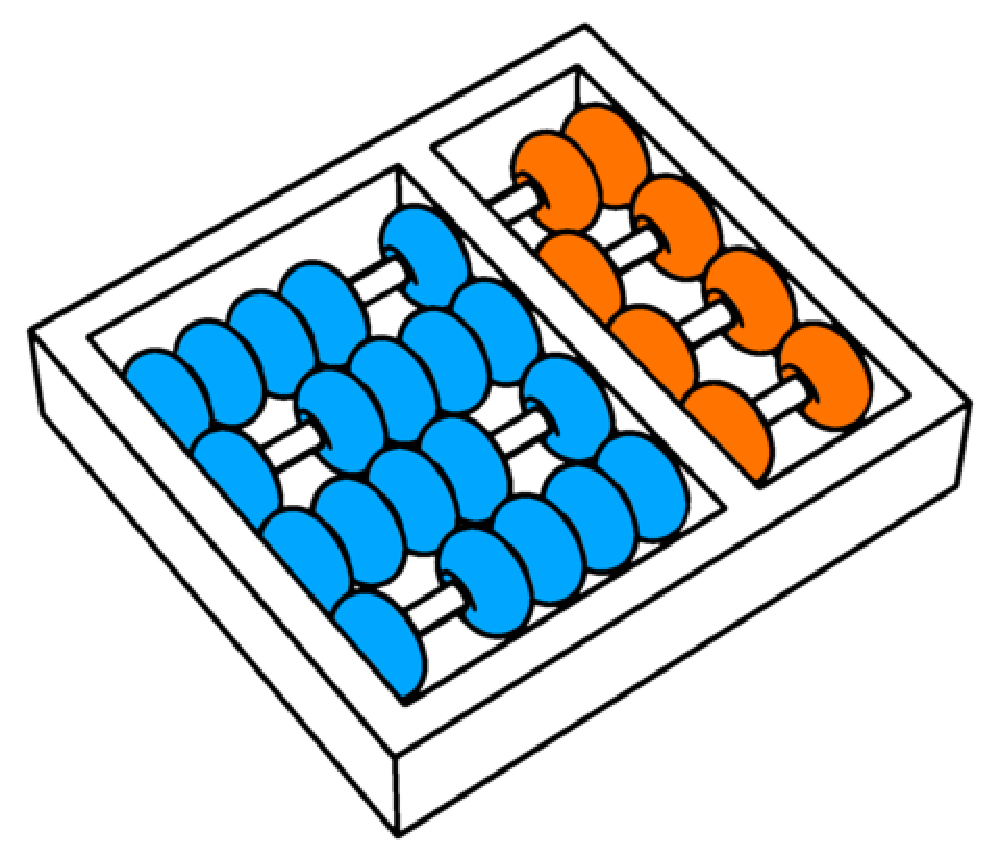
\includegraphics{abaco.pdf}}
}

\institute{Institute of Computing - Unicamp}

\date{November 29, 2013}

\subject{Talks}

\def\defn#1{{\color{red} #1}}
% Insere o numero da pagina no rodape.

\setbeamertemplate{headline}[text line]{%
  \parbox{\linewidth}{\vspace*{8pt}\hfill\insertsection}}

\setbeamertemplate{footline}[text line]{%
  \parbox{\linewidth}{\vspace*{-8pt}\logounicamp\hfill\institute\hfill\inserttitle
  \hfill\logoabaco\hfill\insertpagenumber}}
\setbeamertemplate{navigation symbols}{}

\author{Adriano Ruggero, Gabriel Rodrigues, Mário Brito, Maurício Perez}

  \addtocounter{framenumber}{-1}% If you don't want them to affect the slide number


\addto\captionsportuguese{
\renewcommand{\figurename}{Figure}
\renewcommand{\tablename}{Table}
}

\begin{document}

\begin{frame}
  \titlepage
\end{frame}

\begin{frame}
  \frametitle{Outline}
  \tableofcontents
\end{frame}

\begin{frame}

\begin{block}{Motivation}
\section{Motivation}
\begin{itemize}

\item We (still) live in a ''paper era''

\item Documents forgery has become common

\item There is a way to relate a document to a specific printer?

\end{itemize}

\end{block}


\begin{figure}[!htb]
\centering
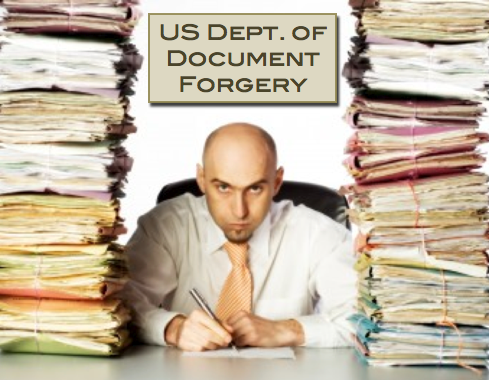
\includegraphics[scale=0.28]{forgery}
\label{fig:forgery}
\caption{Document forgery\footnote{The Infothority\cite{forgery}}}
\end{figure}
{\let\thefootnote\relax\footnotetext{}}
\end{frame}

\begin{frame}
\section{Introduction}
\begin{block}{Printer attribution}

A way to do this is called ''Printer Attribution''

\end{block}

\end{frame}

\begin{frame}

\begin{block}{Methods}

\begin{itemize}

\item Geometric distortion

\item Texture analysis of characters

\end{itemize}

\end{block}

\end{frame}

\begin{frame}

\begin{block}{Geometric distortion}

\begin{figure}[!htb]
\centering
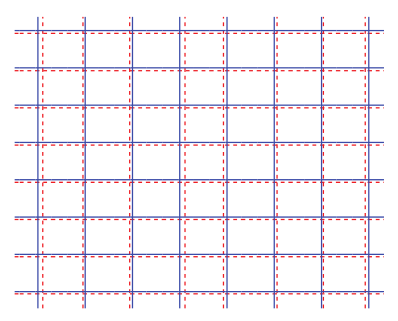
\includegraphics[scale=0.35]{geometric_distortion}
\label{fig:geometric_distortion}
\caption{Geometric distortion \footnote{Geometric Distortion Signatures for Printer Identification\cite{Geometric_Distortion}}}
\end{figure}

\end{block}

{\let\thefootnote\relax\footnotetext{}}

\end{frame}

\begin{frame}

\begin{block}{Texture analysis of characters}

\begin{figure}[!htb]
\centering
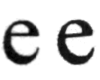
\includegraphics[scale=2]{characters}
\label{fig:characters}
\end{figure}

\end{block}

\end{frame}

\begin{frame}
\section{State-of-the-art}
\begin{block}{State-of-the-art}

\begin{itemize}

\item \textbf{Bulan et al\footnote{Geometric Distortion Signatures for Printer Identification\cite{Geometric_Distortion}}:} a method for
analyzing geometric distortions introduced during the printing process of electrophotographic printers (EP).

\item \textbf{Kee and Farid\footnote{Printer Profiling for Forensics and Ballistics\cite{Printer_Profiling}}:} a method of geometric modeling of degradation caused by the printer.

\end{itemize}

\end{block}
{\let\thefootnote\relax\footnotetext{}}
\end{frame}

\begin{frame}
\section{Proposed solution}
\begin{block}{Proposed solution}

\begin{itemize}

\item Get the image of characters selected from scanned documents (grayscale)

\item Create a co-occurrence matrix

\item Extract its properties (contrast, correlation, energy and homogeneity)

\item Create a feature vector from this properties

\item Use machine learning algorithms to classify them

\end{itemize}

\end{block}

\end{frame}

\begin{frame}

\begin{block}{Printers}

\begin{table}
\caption{Printers used in this work}
\label{tab:printers}
\begin{small}
\begin{center}
\begin{tabular}{ | c | c | c | c |}
\hline
Printer & Documents & Characters ''e'' & Characters ''t'' \\ \hline
Brother-HL4070CDW & 28 & 252 & 252\\
Canon-D1150 & 28 & 252 & 252\\
Canon-MF3240 & 28 & 252 & 252\\
Canon-MF4370DN & 27 & 252 & 252 \\
HP-CLJ-CP2025A & 28 & 252 & 252\\
Lexmark-E260D & 28 & 252 & 252\\
\hline
\end{tabular}
\end{center}   
\end{small} 
\end{table}

\end{block}

\end{frame}

\begin{frame}

\begin{block}{Characters}

\begin{itemize}

\item Characters ''e'' and ''t'' (most common in English texts)

\item Same size, same font, no texts effects

\item Misaligned characters were summarily discarded

\end{itemize}

\end{block}

\end{frame}

\begin{frame}

\begin{block}{Differences between aligned and misaligned characters}

\begin{table}
\label{tab:properties_differences}
\caption{Differences between an original character and a rotated character.}
\begin{center}
\begin{tabular}{l*{3}{c}r}
Property & Original character & Rotated character (-4º) \\
\hline
Contrast & 3.2443 - 2.2905 & 5.1617 - 4.6504 \\
Correlation & 0.7869 - 0.8502 & 0.6967 - 0.7264 \\
Energy & 0.1608 - 0.1744 & 0.1106 - 0.1216 \\
Homogeneity & 0.6946 - 0.7462 & 0.6610 - 0.6995 \\
\end{tabular}
\end{center}
\end{table}

\end{block}

\end{frame}

\begin{frame}

\begin{block}{Something about printers}

\begin{itemize}

\item All documents came from laser printers, so...\pause

\begin{itemize}

\item we need to understand how they works!

\end{itemize}

\end{itemize}

\end{block}

\end{frame}

\begin{frame}

\begin{block}{Default laser printer schema}

\begin{figure}[!htb]
\centering
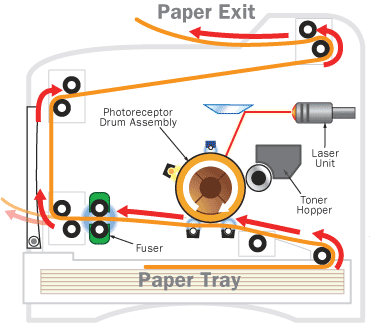
\includegraphics[scale=0.4]{page_printer}
\label{fig:page_printer}
\caption{Default laser printer schema\footnote{Forensic Document Examination Services\cite{Page_printer}}}
\end{figure}

\end{block}
{\let\thefootnote\relax\footnotetext{}}
\end{frame}

\begin{frame}

\begin{block}{Division of document areas}

\begin{figure}[!htb]
\centering
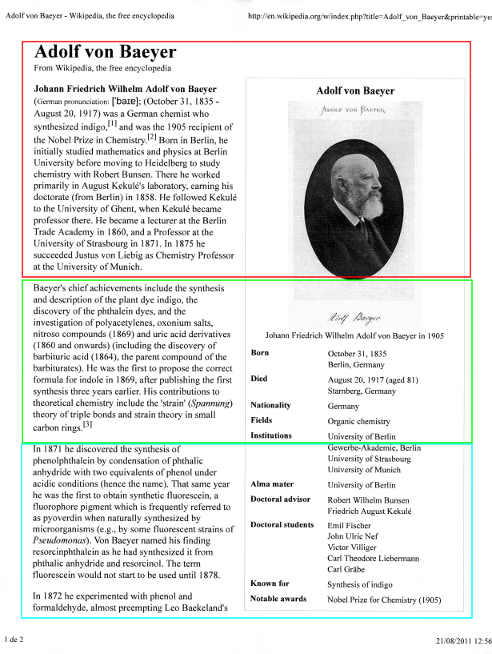
\includegraphics[scale=0.3]{document_areas}
\label{fig:document_areas}
\end{figure}

\end{block}

\end{frame}

\begin{frame}

\begin{block}{Gray level co-occurrence matrix}

The primary use of the co-occurrence matrix is characterized texture in an image from a set of statistics for instances of each gray level in different pixels
along different directions\footnote{Classificação de texturas a partir de vetores de atributos e função de distribuição de probabilidades\cite{Rocha}}.

\end{block}

\begin{block}{In other words...}

\begin{itemize}

\item A matrix of relative frequencies $P (i, j, d, \theta)$

\begin{itemize}

\item $p$ represents the pixel-of-interest

\item $i$ and $j$ represents the properties

\item $\theta$ represents the distance

\end{itemize}

\end{itemize}

\end{block}

{\let\thefootnote\relax\footnotetext{}}

\end{frame}

\begin{frame}
\section{Experiments and discussion}

\begin{block}{Character's selection and extraction}

\begin{figure}[!htb]
\centering
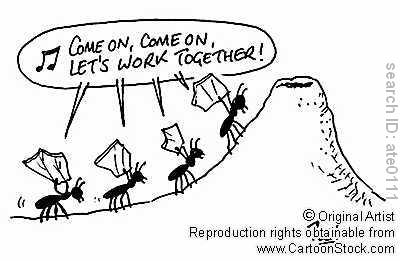
\includegraphics[scale=0.5]{ants}
\label{fig:ants}
\caption{An ant's work!\footnote{The Wifey Journals\cite{Ants}}}
\end{figure}

\end{block}
{\let\thefootnote\relax\footnotetext{}}
\end{frame}

\begin{frame}

\begin{block}{Neighborhood}

\begin{figure}[!htb]
\centering
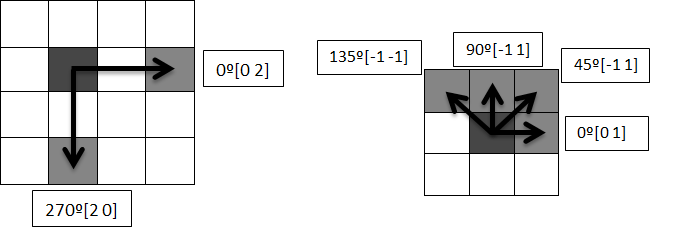
\includegraphics[scale=0.3]{neighbor}
\label{fig:neighbor}
\caption{Neighborhood A, leftmost, and B, rightmost, used in
properties extraction.}
\end{figure}

\end{block}

\end{frame}

\begin{frame}

\begin{block}{Algorithms versus correct classification}

\begin{table}
\label{tab:correct_classification}
\caption{Percentage of correct classifications of printers.}
\begin{center}
\begin{small} 
\setlength{\tabcolsep}{3pt} 
\begin{tabular}{l*{5}{c}r} & \multicolumn{2}{c}{Neighborhood A} & \multicolumn{2}{c}{Neighborhood B}\\ \cline{1-5}
Method & Chars e’s & Chars t’s & Chars e’s & Chars t’s \\
\hline
Logistic & 81 & 81.3 & 85 & 84.6\\
KStar & 77.6 & 83 & 72 & 79.6\\
RotationForest & 83.1 & 85 & 81.7 & 85.7\\
NNge & 74.1 & 80.2 & 72.2 & 67.8\\
LMT & 83.8 & 84.6 & 82.7 & 85.5\\

\end{tabular}
\end{small}
\end{center}
\end{table}

\end{block}

\end{frame}

\begin{frame}

\begin{block}{Printer attribution results}

\begin{table}
\caption{Percentage of correct printer attribution.}
\label{tab:correct_printer_attribution}
\begin{center}
\begin{small} 
\setlength{\tabcolsep}{3pt} 
\begin{tabular}{l*{4}{c}r} \cline{1-4}
Method & Chars e’s & Chars t’s & Chars e’s and t’s \\
\hline
Logistic & 21/24 = 87.5\% & 22/24 = 91.7\% & 21/24 = 87.5\% \\

RotationForest & 21/ 24 = 87.5\% & 21/24 = 87.5\% & 22/24 = 91.7\% \\

LMT & 21/24 = 87.5\% & 21/24 = 87.5\% & 22/24 = 91.7\% \\

\end{tabular}
\end{small}
\end{center}
\end{table}

\end{block}

\end{frame}

\begin{frame}
\section{Conclusions and future work}

\begin{block}{Conclusions}

\begin{itemize}

\item Is possible assign a document to a printer analyzing the texture of its characters

\item Greater feature vectors doesn’t mean a better classifier

\item Character choice would have probably low impact on the results

\end{itemize}

\end{block}

\end{frame}

\begin{frame}

\begin{block}{Future work}

\begin{itemize}

\item Extract more varied or more characters

\item Try other texture analyzers, such as HOG (Histograms of Oriented Gradients Extract) or LBP (Local Binary Patterns), and no GLCM.

\item A (semi) automated method to extract the characters would be of great benefit to researchers in this field.

\end{itemize}

\end{block}

\end{frame}

\begin{frame}
\section{Acknowledgements}

\begin{block}{Acknowledgements}

\begin{itemize}

\item Professor Anderson Rocha

\item Giuliano Pinheiro

\end{itemize}

\end{block}

\end{frame}

\section{References}
\begin{frame} [allowframebreaks]

\frametitle{Bibliography}

\bibliographystyle{unsrt}
\bibliography{ref_presentation}

\end{frame}

%%%%% Thanks page
\section{}
\begin{frame}
\frametitle{Thanks}
\vskip30pt

\begin{center}
{\bf \color{alert} Thanks!}
\end{center}

\vskip30pt

\begin{center}

\vskip12pt

Adriano R. Ruggero, Gabriel Rodrigues, Mário F. Brito, Maurício L. Perez

\end{center}

%%\titlepage
\end{frame}

\end{document}